{
\setbeamertemplate{footline}{}
\appendix
\section{Приложение}

\begin{frame}[t,noframenumbering]{Приложение: историческая декомпозиция $M2$}
\vspace{-0.25cm}
\centering
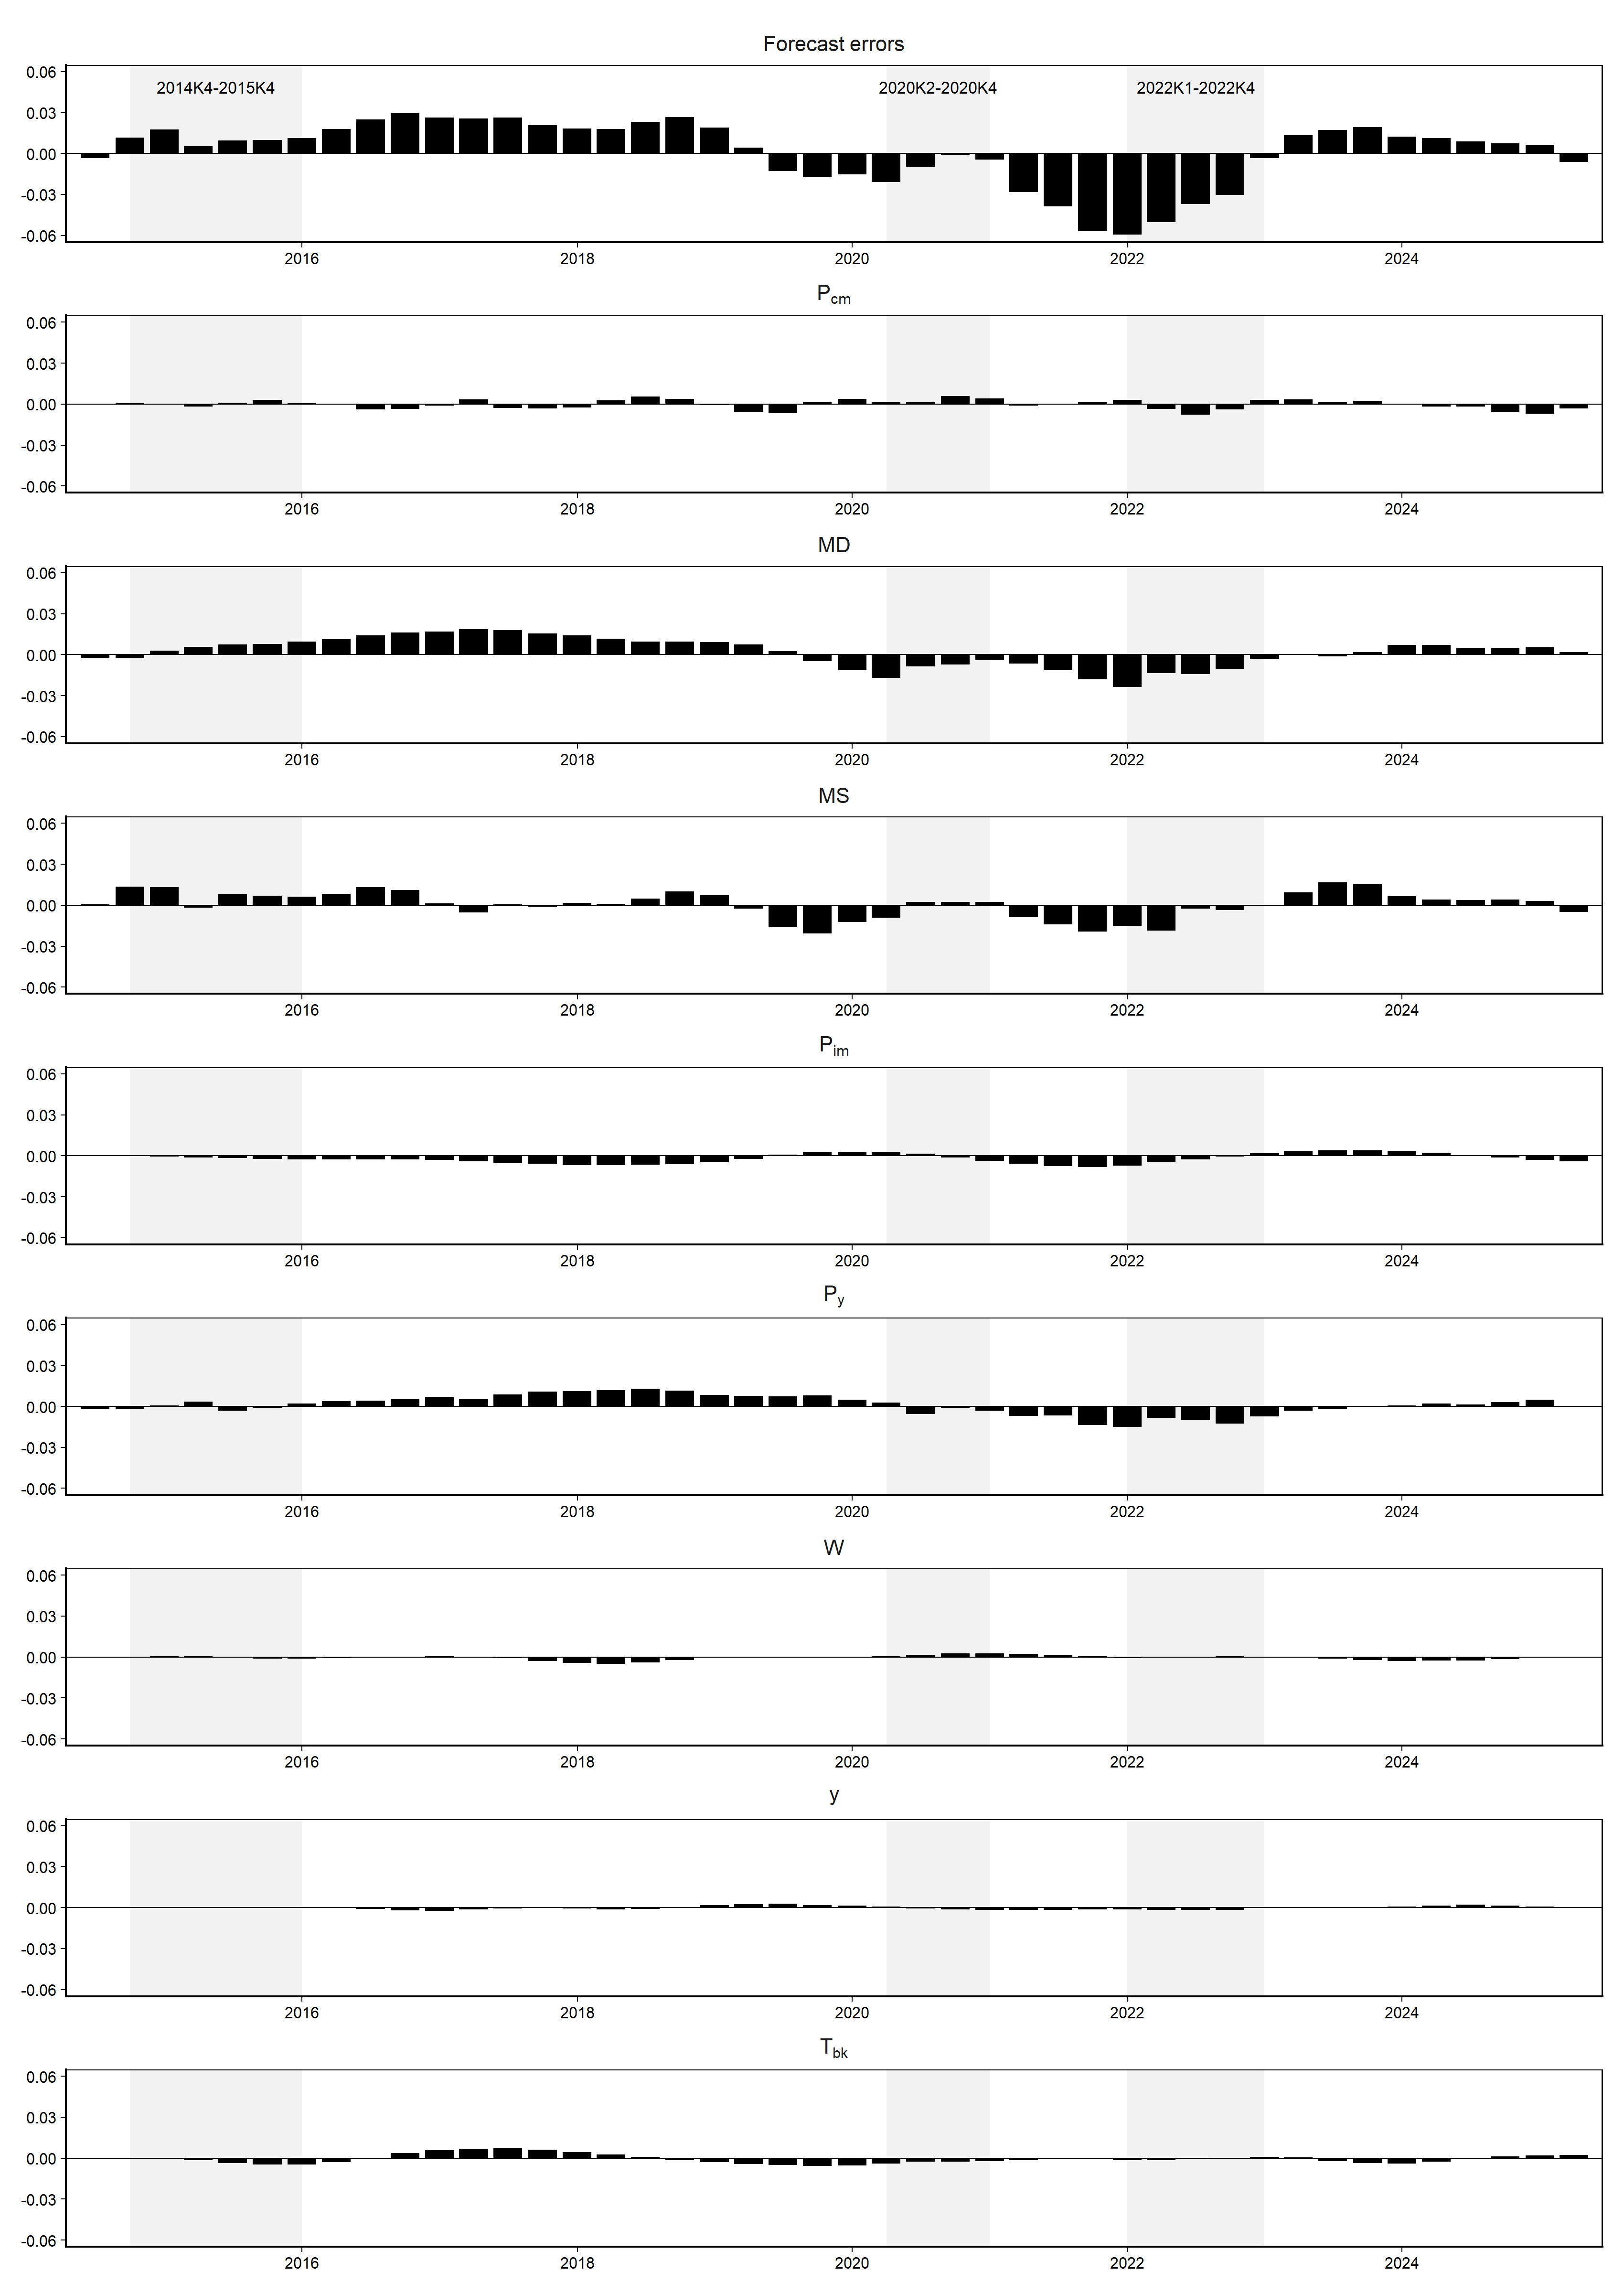
\includegraphics[
    width=\textwidth,
    height=0.84\textheight,
    keepaspectratio
]{historical_decomposition_m2.png}
\end{frame}

\begin{frame}[t,noframenumbering]{Приложение: историческая декомпозиция $R$}
\vspace{-0.25cm}
\centering
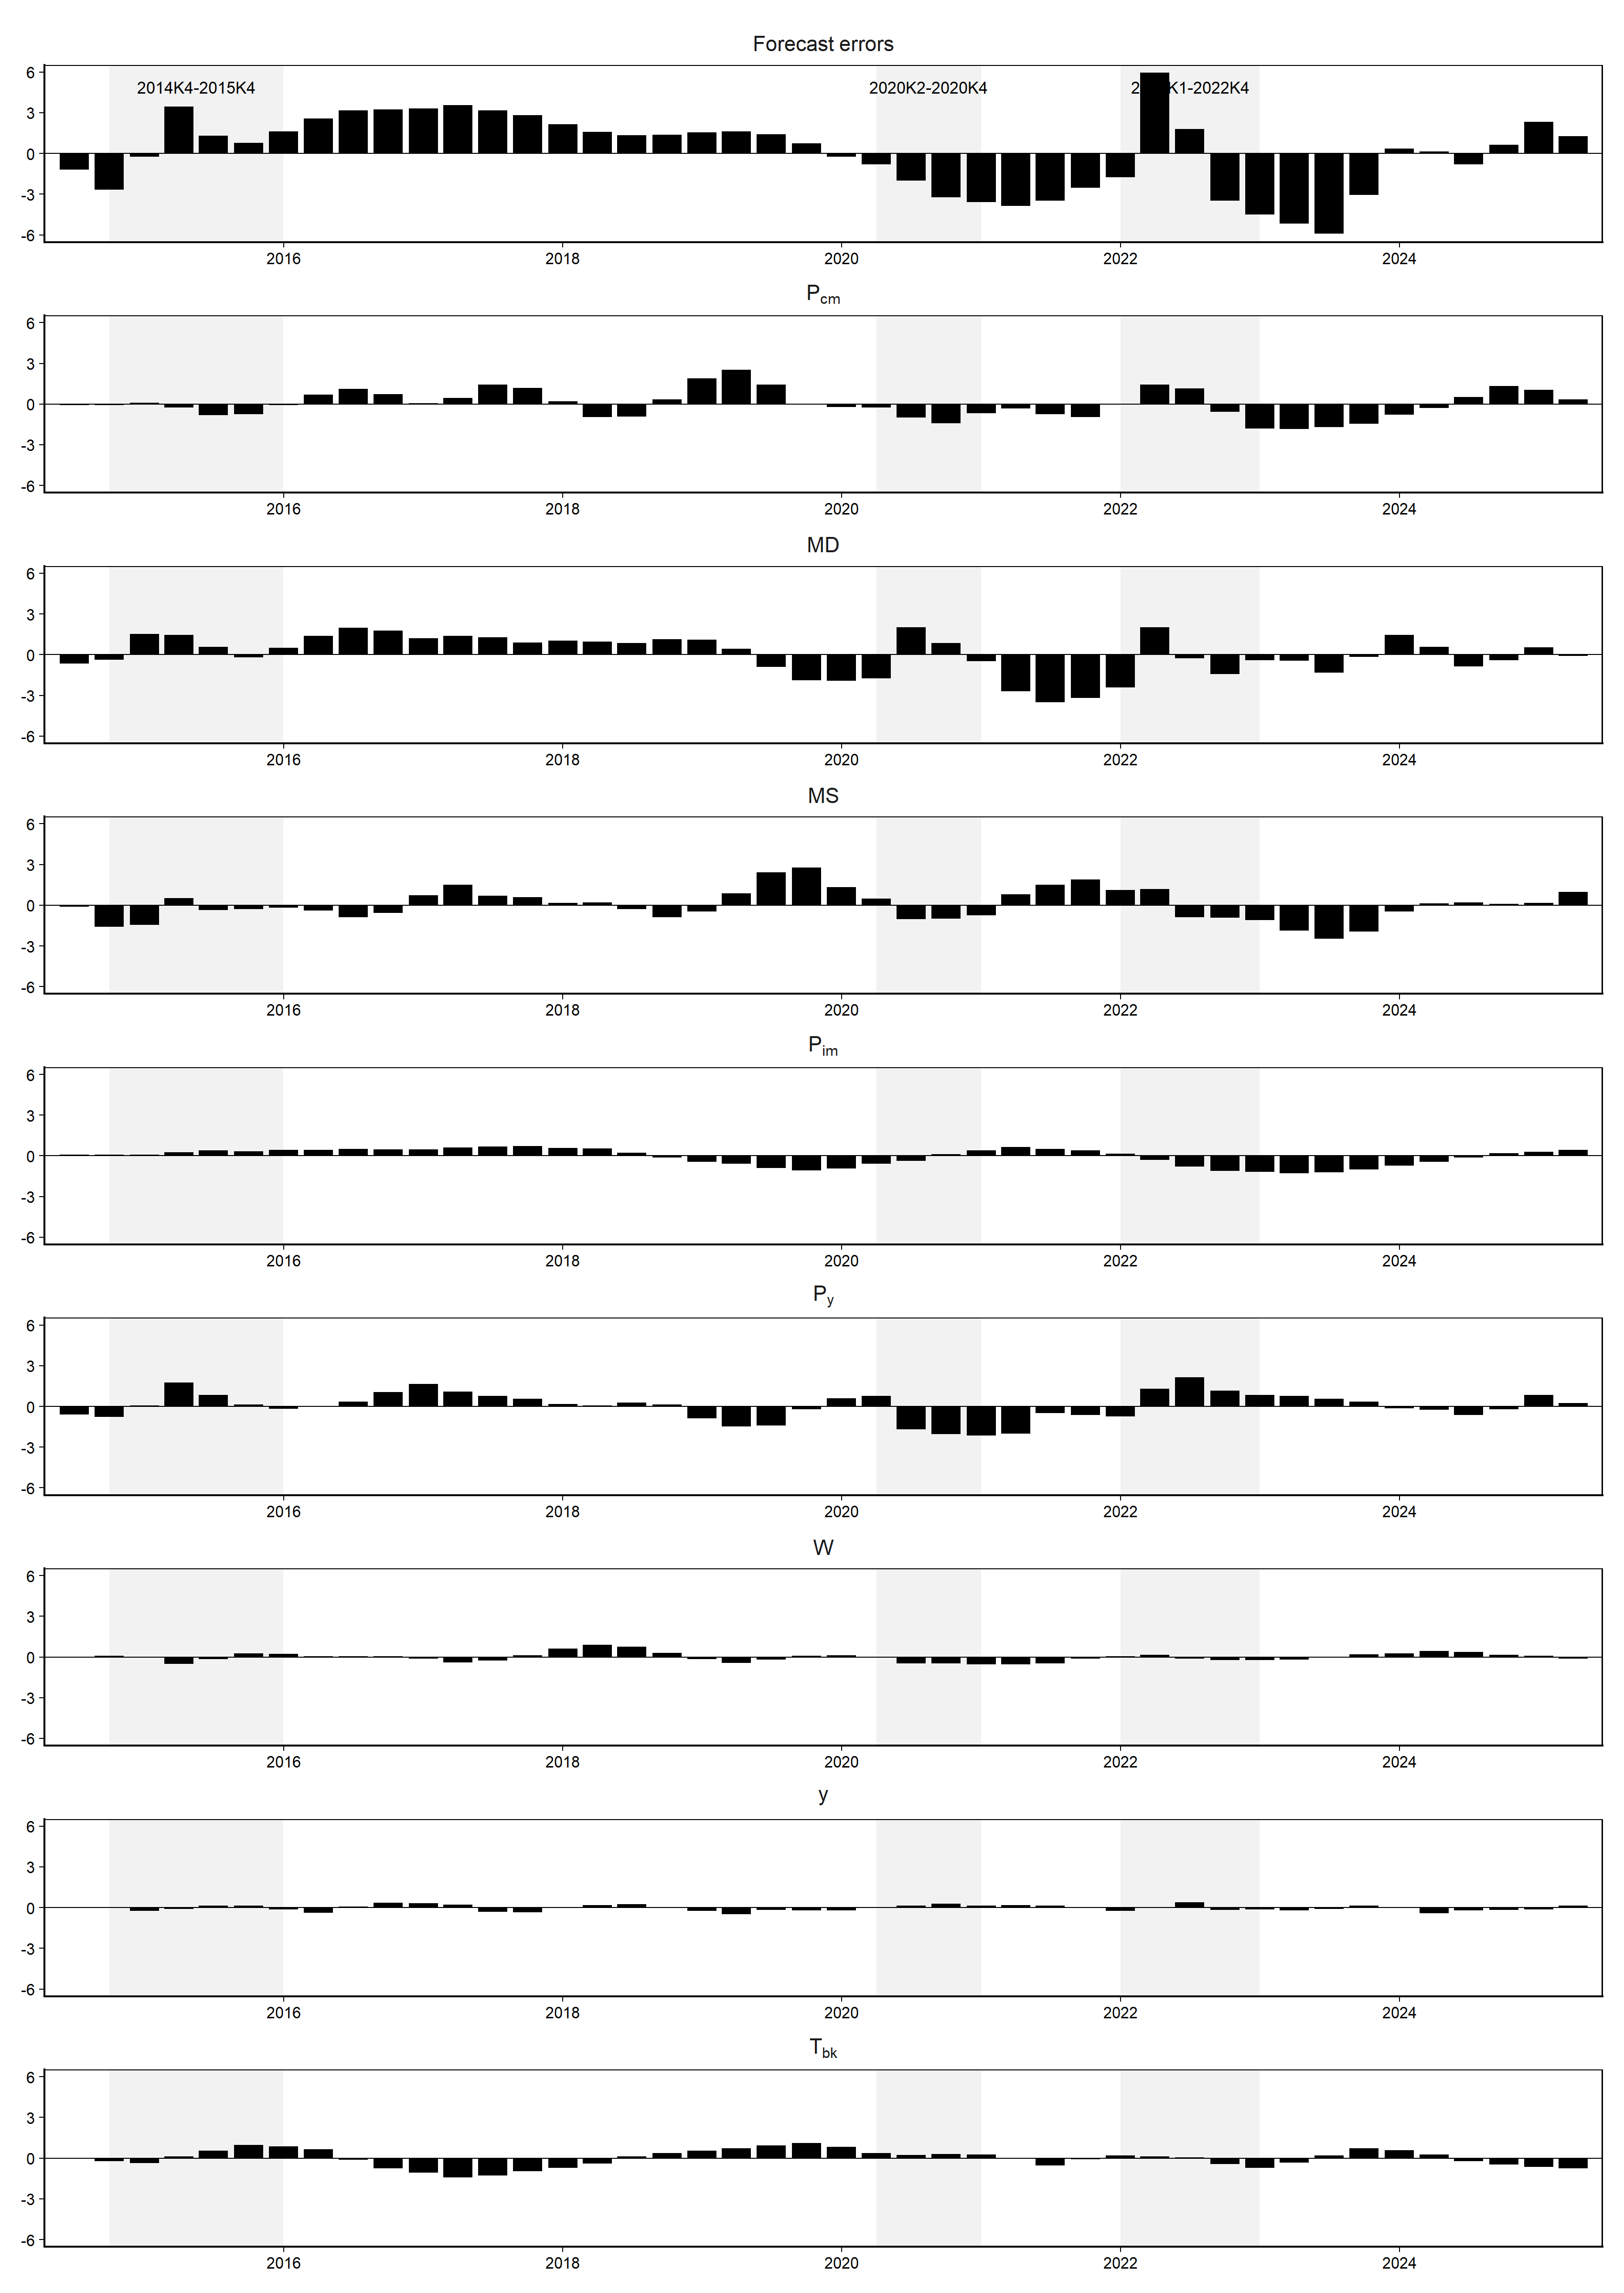
\includegraphics[
    width=\textwidth,
    height=0.84\textheight,
    keepaspectratio
]{historical_decomposition_key_rate.png}
\end{frame}

\begin{frame}[t,noframenumbering]{Приложение: историческая декомпозиция $P_y$}
\vspace{-0.25cm}
\centering
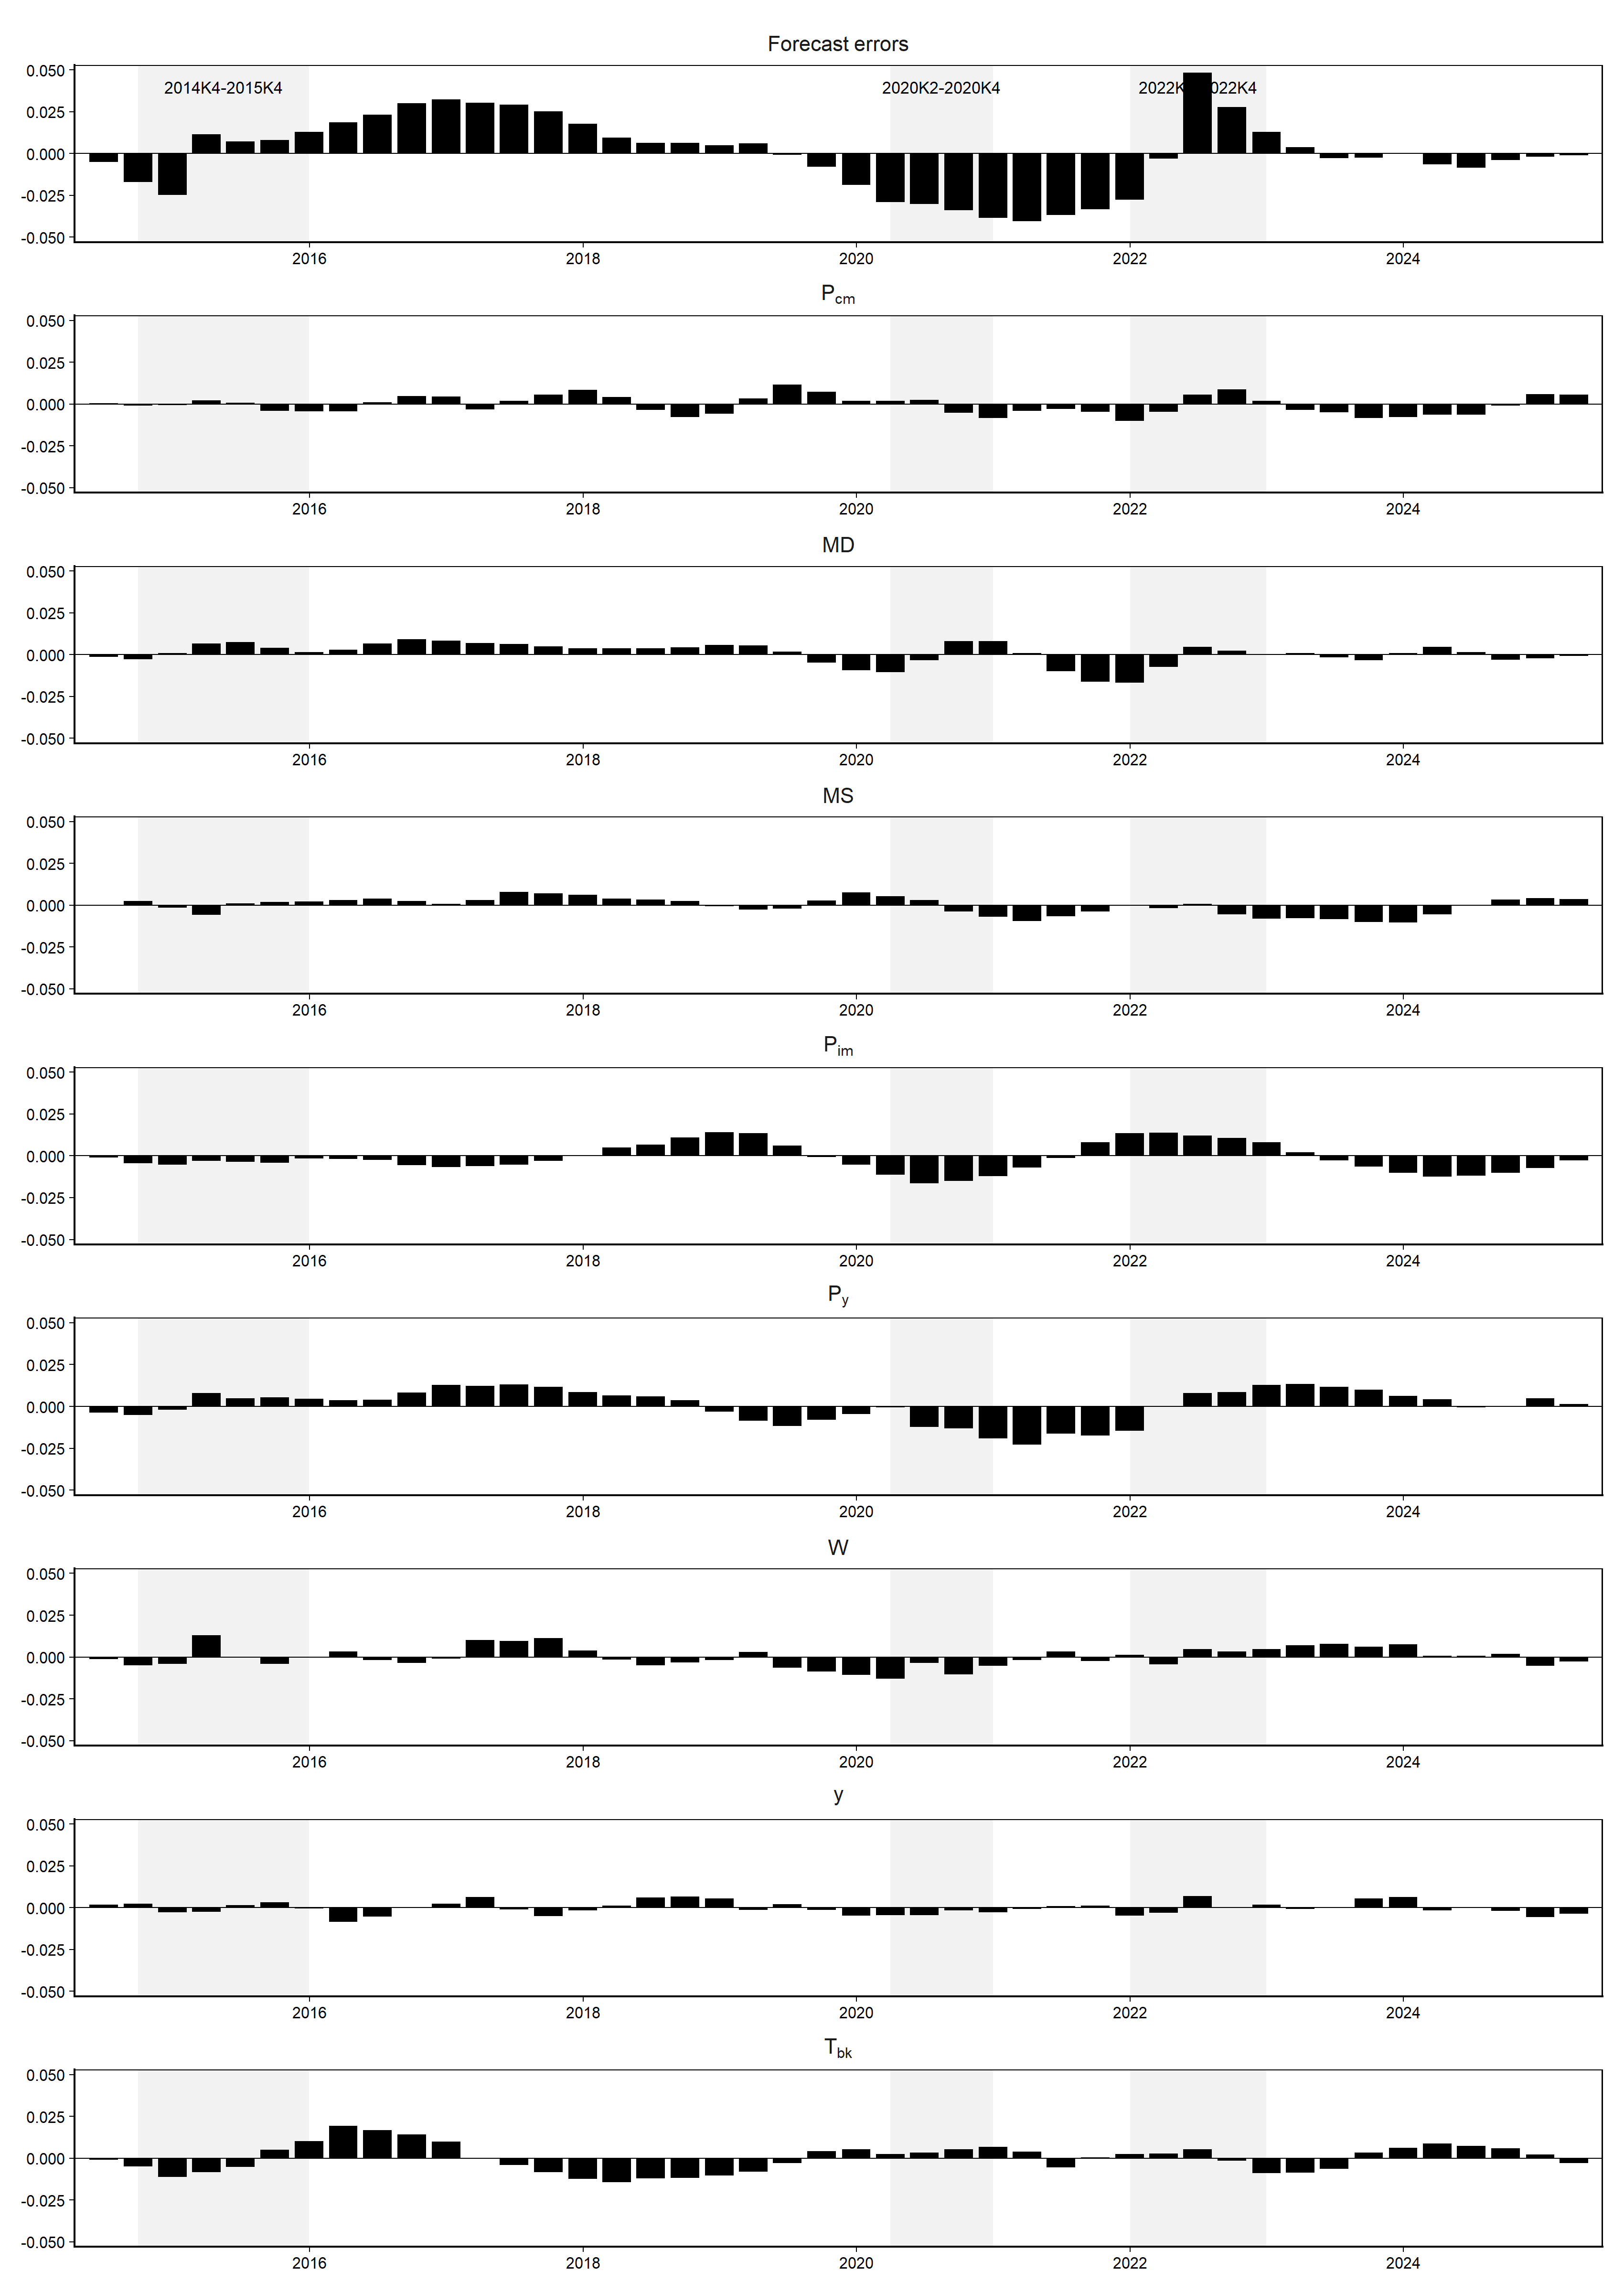
\includegraphics[
    width=\textwidth,
    height=0.84\textheight,
    keepaspectratio
]{historical_decomposition_cpi.png}
\end{frame}

\begin{frame}[t,noframenumbering]{Приложение: историческая декомпозиция $y$}
\vspace{-0.25cm}
\centering
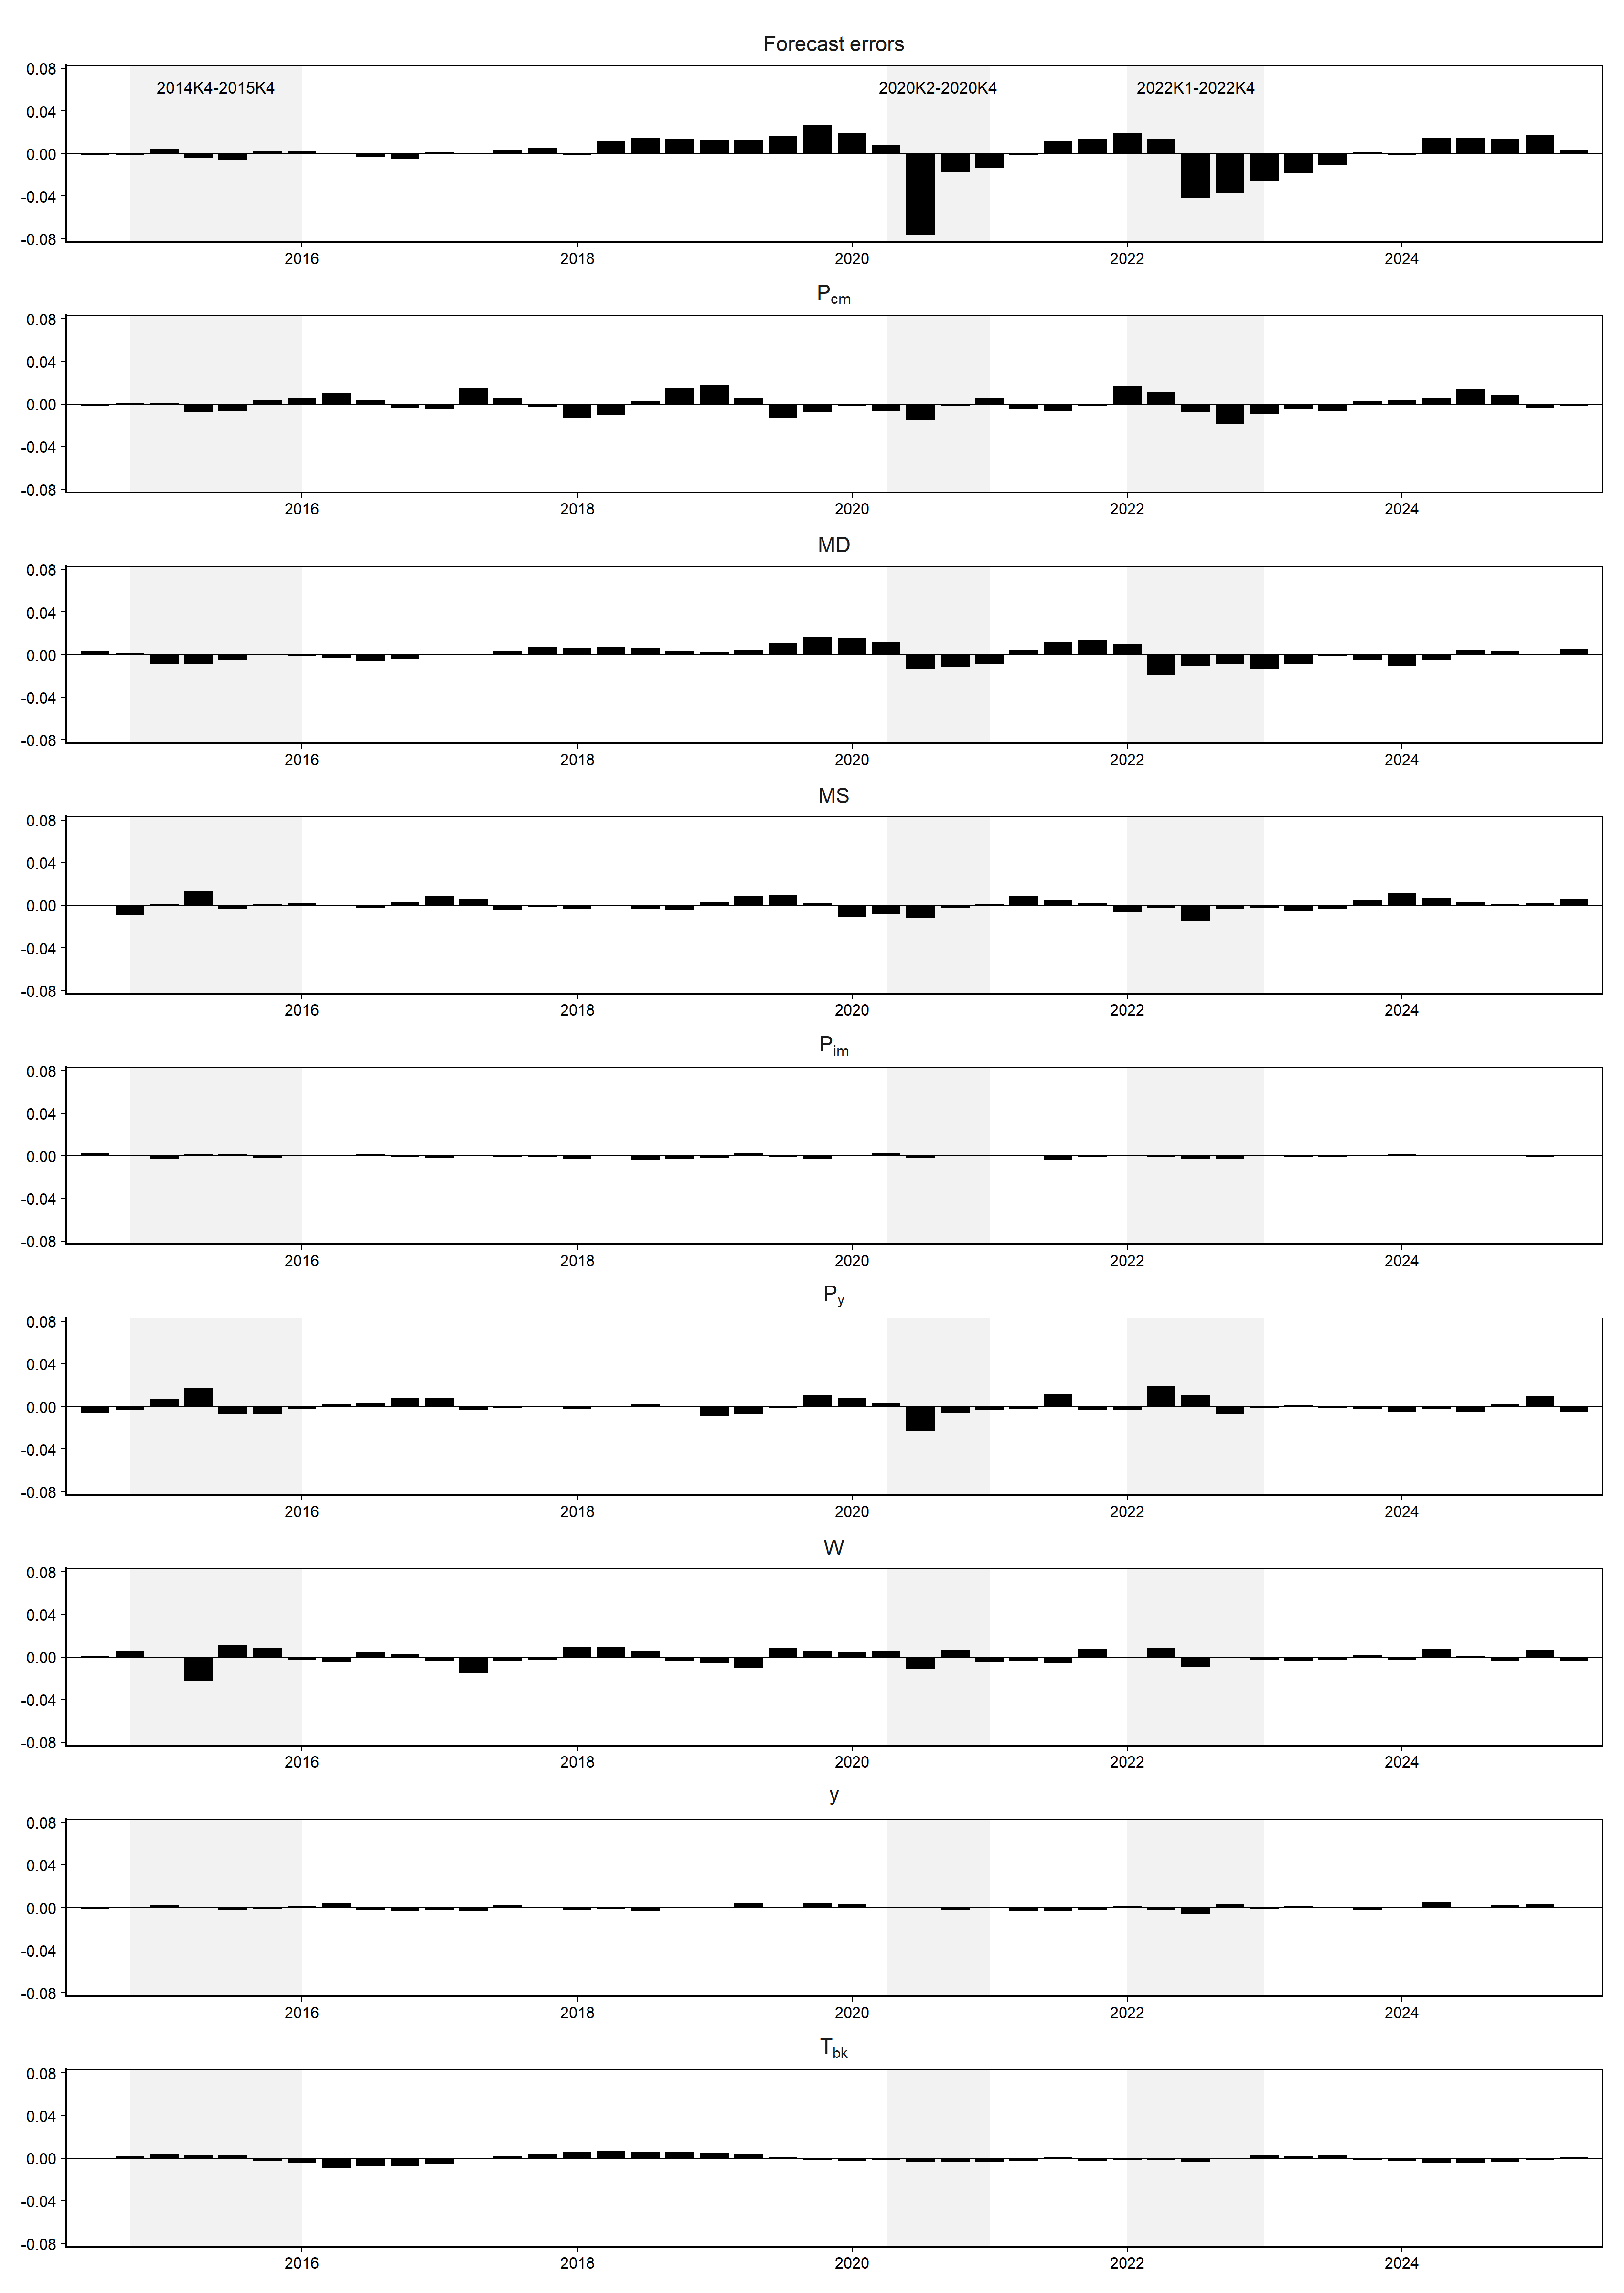
\includegraphics[
    width=\textwidth,
    height=0.84\textheight,
    keepaspectratio
]{historical_decomposition_gdp.png}
\end{frame}

\begin{frame}[t,noframenumbering]{Приложение: структурные шоки, часть 1}
\vspace{-0.25cm}
\centering
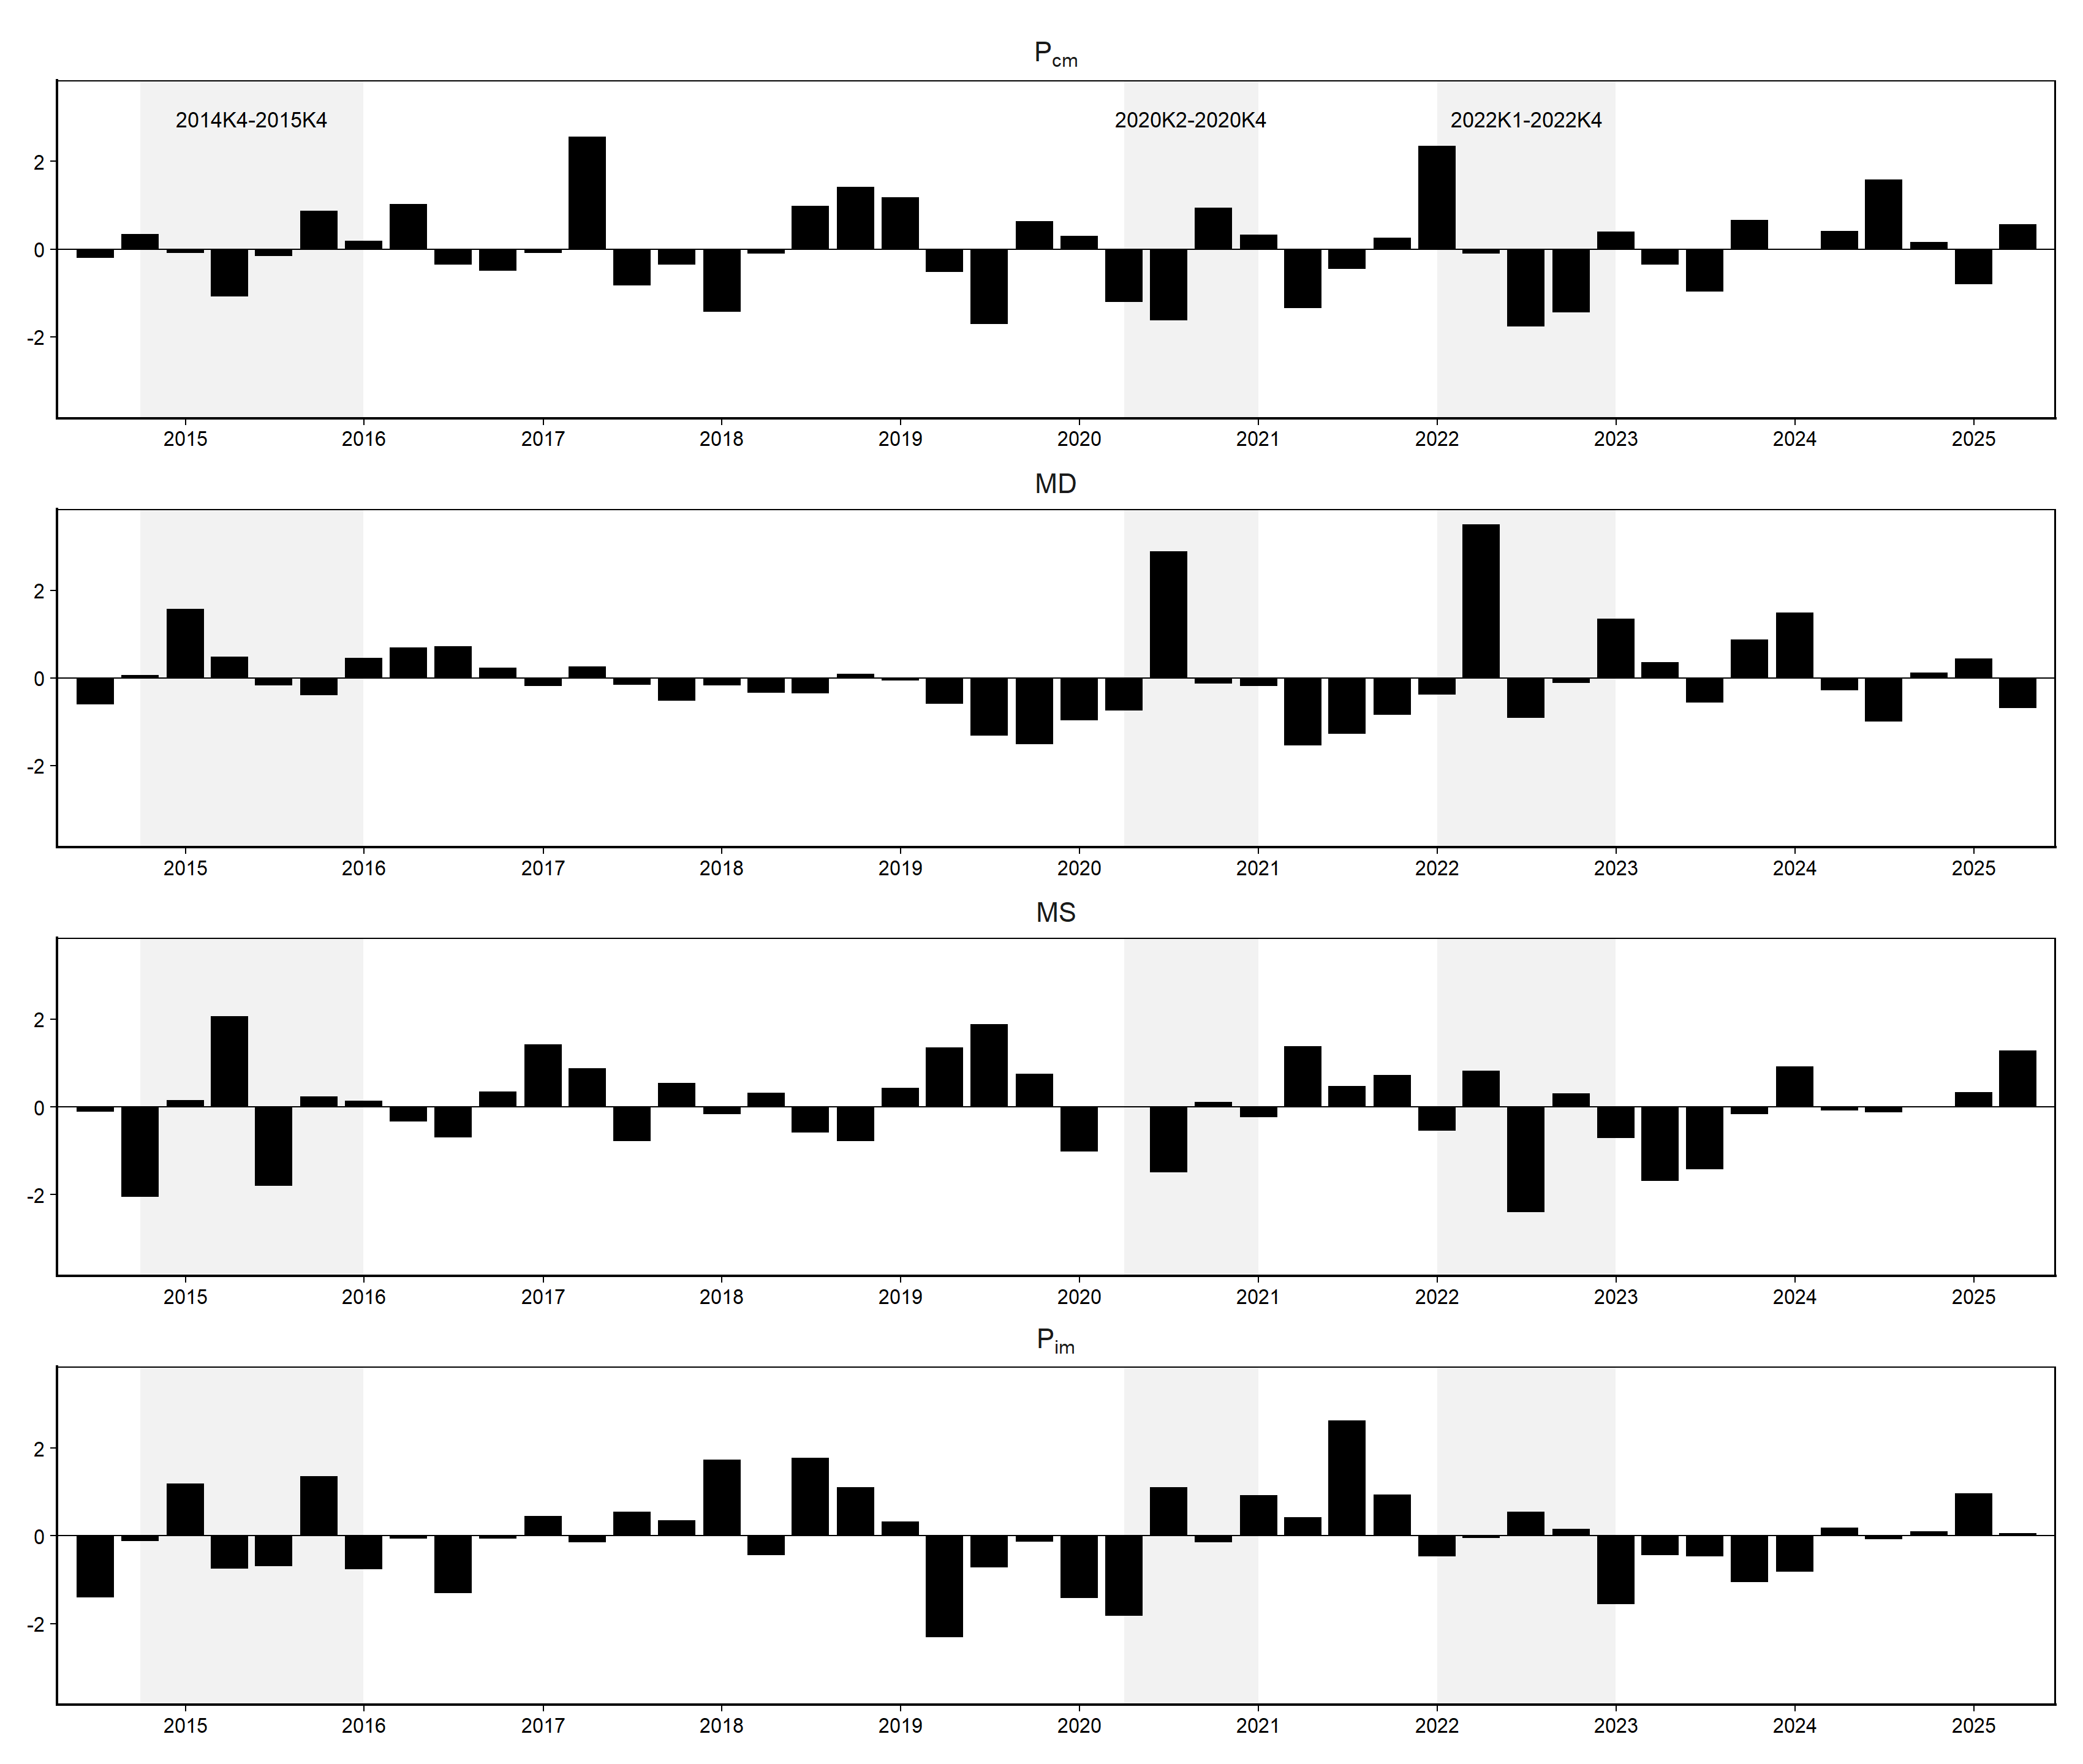
\includegraphics[
    width=\textwidth,
    height=0.84\textheight,
    keepaspectratio
]{structural_shocks_8a.png}
\end{frame}

\begin{frame}[t,noframenumbering]{Приложение: структурные шоки, часть 2}
\vspace{-0.25cm}
\centering
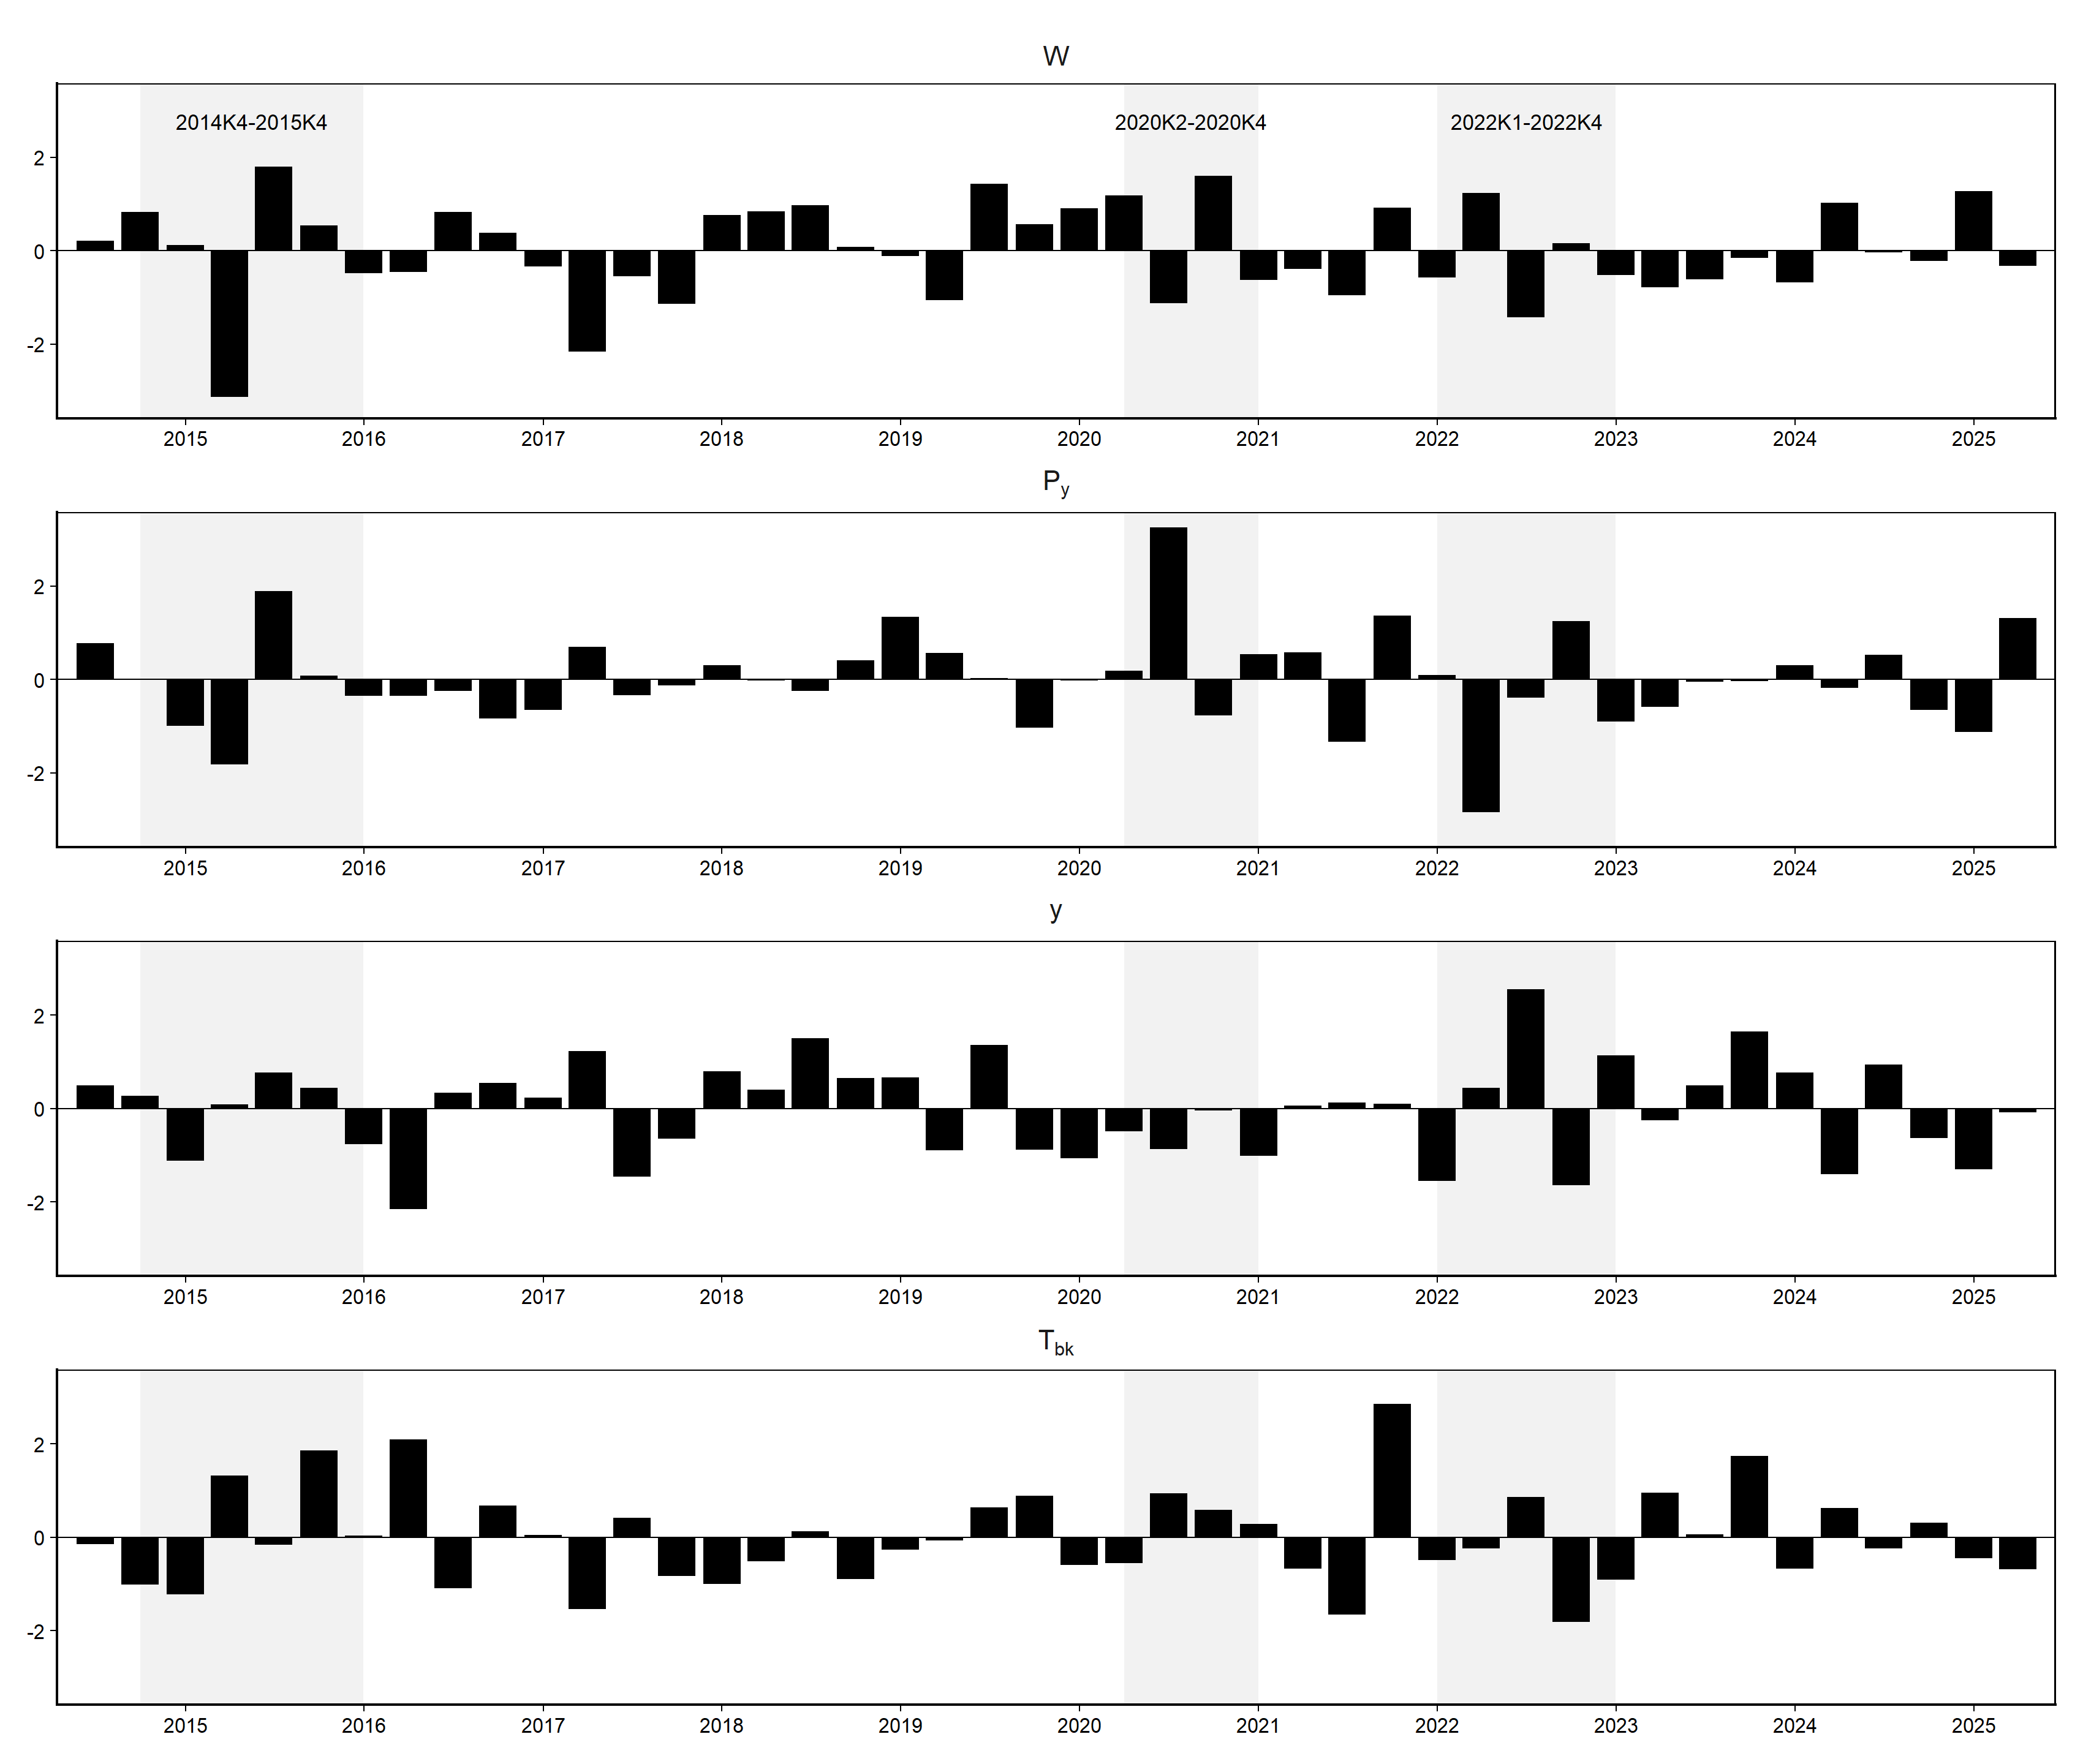
\includegraphics[
    width=\textwidth,
    height=0.84\textheight,
    keepaspectratio
]{structural_shocks_8b.png}
\end{frame}

% \begin{frame}[t,noframenumbering]{Приложение: спецификация VAR/SVAR}
% \vspace{-0.15cm}
% \centering
% \scriptsize
% \setlength{\tabcolsep}{4pt}
% \renewcommand{\arraystretch}{0.95}
% \begin{tabular}{ll}
\toprule
item & value\\
\midrule
frequency & quarterly\\
sample period & 2014Q1--2025Q1\\
observations after lags & 44\\
lag order & p = 1\\
variables & Pcm, M2, R, Pim, Py, W, y, OvDeb\\
\addlinespace
transformations & log-levels for level variables; R without log\\
model type & VAR(1) / SVAR(1)\\
\bottomrule
\end{tabular}

% \end{frame}

\begin{frame}[t,noframenumbering]{Приложение: информационные коэффициенты}
\vspace{-0.15cm}
\centering
\scriptsize
\setlength{\tabcolsep}{4pt}
\renewcommand{\arraystretch}{0.95}
\begin{tabular}{rrrrr}
\toprule
lag & AIC & HQ & SC & FPE\\
\midrule
1 & -54.282 & -53.177 & -51.147 & 0.000\\
2 & -54.542 & -52.455 & -48.621 & 0.000\\
3 & -57.754 & -54.684 & -49.046 & 0.000\\
4 & -200.140 & -196.088 & -188.646 & 0.000\\
5 & Inf & Inf & Inf & 0.000\\
\addlinespace
6 & Inf & Inf & Inf & 0.000\\
7 & Inf & Inf & Inf & 0.000\\
8 & Inf & Inf & Inf & 0.000\\
\bottomrule
\end{tabular}

\end{frame}

\begin{frame}[t,noframenumbering]{Приложение: устойчивость VAR}
\vspace{-0.15cm}
\centering
\scriptsize
\setlength{\tabcolsep}{6pt}
\renewcommand{\arraystretch}{0.95}
\begin{tabular}{lr}
\toprule
root\_id & modulus\\
\midrule
1 & 1.018\\
2 & 0.985\\
3 & 0.751\\
4 & 0.751\\
5 & 0.659\\
\addlinespace
6 & 0.659\\
7 & 0.451\\
8 & 0.451\\
stable & FALSE\\
\bottomrule
\end{tabular}

\end{frame}


}